% This is samplepaper.tex, a sample chapter demonstrating the
% LLNCS macro package for Springer Computer Science proceedings;
% Version 2.25 of 2026/09/03
%
\documentclass[runningheads]{llncs}
%
\usepackage[T1]{fontenc}
% T1 fonts will be used to generate the final print and online PDFs,
% so please use T1 fonts in your manuscript whenever possible.
% Other font encondings may result in incorrect characters.
%

\usepackage{amsmath}         % must be loaded before newtxmath
\usepackage{newtxtext}       %
\usepackage[varvw]{newtxmath}       % selects Times Roman as basic font


\usepackage{graphicx}
% Used for displaying a sample figure. If possible, figure files should
% be included in EPS format.
%
\usepackage{booktabs}
\usepackage{multirow}
\usepackage{xcolor}
\usepackage{tikz}
\usetikzlibrary{positioning, arrows.meta, matrix, calc}
\usepackage{pgfplots}
\pgfplotsset{compat=1.18}
\usepgfplotslibrary{groupplots}
% Chart colours: one fixed colour per model (checked for colour-vision
% deficiency on white), a blue/neutral/red scale for the quality tiers, and ink.
\definecolor{cQwen}{HTML}{2A78D6}
\definecolor{cLlama}{HTML}{EB6834}
\definecolor{cDeepSeek}{HTML}{1BAF7A}
\definecolor{cInclude}{HTML}{2A78D6}
\definecolor{cFlag}{HTML}{C3C2B7}
\definecolor{cExclude}{HTML}{E34948}
\definecolor{cSeq}{HTML}{184F95}
\definecolor{cInk}{HTML}{0B0B0B}
\definecolor{cInk2}{HTML}{52514E}
\definecolor{cAxis}{HTML}{C3C2B7}
\definecolor{cGrid}{HTML}{E1E0D9}
\newcommand{\tierkey}[1]{\textcolor{#1}{\rule{5pt}{5pt}}}
\pgfplotsset{paperaxis/.style={
  tick label style={font=\scriptsize, color=cInk2}, label style={font=\scriptsize},
  title style={font=\scriptsize, yshift=-2pt}, axis line style={cAxis},
  every tick/.style={cAxis}, major tick length=2pt, grid=major,
  grid style={cGrid, line width=0.3pt}}}
\usepackage[most]{tcolorbox}
%
% If you use the hyperref package, please uncomment the following two lines
% to display URLs in blue roman font according to Springer's eBook style:
\usepackage[hidelinks]{hyperref}
\usepackage{color}
\renewcommand\UrlFont{\color{blue}\rmfamily}
\urlstyle{rm}
\usepackage{cleveref}
\crefname{section}{Sect.}{Sects.}
\Crefname{section}{Section}{Sections}
\crefname{figure}{Fig.}{Figs.}
\Crefname{figure}{Fig.}{Figs.}
\crefname{table}{Table}{Tables}
\crefname{equation}{Eq.}{Eqs.}
%
\begin{document}
%
\title{UzABSA-LLM: Parameter-Efficient Fine-Tuning and Multi-Domain Annotation for Uzbek Aspect-Based Sentiment Analysis}
%
\titlerunning{UzABSA-LLM: Fine-Tuning and Multi-Domain Annotation for Uzbek ABSA}
% If the paper title is too long for the running head, you can set
% an abbreviated paper title here
%
\author{Sanatbek Matlatipov\orcidID{0000-0002-6895-3436}}
%
\authorrunning{S. Matlatipov}
% First names are abbreviated in the running head.
% If there are more than two authors, 'et al.' is used.
%
\institute{Faculty of Applied Mathematics and Intelligent Technologies, National University of Uzbekistan named after Mirzo Ulugbek, Tashkent 100174, Uzbekistan\\
\email{s.matlatipov@nuu.uz}}
%
\maketitle              % typeset the header of the contribution
%
\begin{abstract}
In this paper, we investigate the application of parameter-efficient fine-tuning to scalable aspect-based sentiment analysis (ABSA) of Uzbek business reviews. More concretely, we fine-tune Qwen 2.5-7B, Llama 3.1-8B, and DeepSeek-R1-Distill-7B in one QLoRA setup to perform aspect term extraction and polarities classification in pairs, giving results in the format of structured JSON. Our evaluation is based on a test set of 609 samples taken from the review-grouped and deduplicated split, using zero-shot prompting with the same models as the control condition. As a result of fine-tuning, we obtain nearly double F1 for aspect term extraction and triple F1 for aspect-polarity pair classification: Qwen has the best extraction F1 (0.708) with a 100\% parsing ratio, whereas Llama leads in pair F1 (0.651) and sentiment classification accuracy (0.925). We then compare the performance of our fine-tuned LLMs to that of the fine-tuned 110M-parameter Uzbek BERT encoder on the task of sentiment classification, joint prediction, and aspect extraction. LLMs surpass BERT models in sentiment classification and joint prediction tasks but are comparable in the aspect extraction task. We outline the three-step annotation process: local LLM-based annotation, LLM-as-Judge-based score generation, and aggregation based on quality tiers. This process results in 9,884 aspect-level annotations when used on 5,038 business review documents across 23 domains. The scores generated by the LLM judge panel correlate with the human scores at $\rho=0.78$. Furthermore, we additionally release a reconciled, double-annotated subset of 80 reviews. All code, models, and datasets are publicly released.

\keywords{Aspect-Based Sentiment Analysis \and Uzbek \and Low-Resource NLP \and QLoRA \and Large Language Models \and LLM-as-Judge}
\end{abstract}
%
%
%
\section{Introduction}
\label{sec:intro}
Aspect-based sentiment analysis (ABSA) identifies the aspects of an entity that a text evaluates and the polarity expressed towards each~\cite{pontiki-etal-2014-semeval}. Uzbek, a Turkic language with nearly 38 million speakers,\footnote{\url{https://www.worldometers.info/world-population/uzbekistan-population/}} is poorly served by this line of work: user-generated text mixes Latin and Cyrillic script, agglutinative morphology yields many surface forms per lemma, and the language is thinly represented in multilingual pre-training data. Open-weight 7--8B LLMs such as Qwen~2.5~\cite{Qwen2024-kr}, Llama~3.1~\cite{Grattafiori2024-ka} and the DeepSeek-R1 distillates~\cite{Guo2025} offer cross-lingual transfer, and QLoRA~\cite{3666122.3666563} makes adapting them feasible on a single GPU. We cast ABSA as single-pass generation of a JSON list of aspects and ask three questions:

\begin{itemize}
\item[\textbf{RQ1}] Can QLoRA fine-tuning of an open-weight LLM perform joint aspect extraction and sentiment classification for Uzbek, and how does it compare with zero-shot prompting and fine-tuned monolingual encoders?
\item[\textbf{RQ2}] Under one fixed fine-tuning recipe, does validation loss predict ABSA performance?
\item[\textbf{RQ3}] Can a model fine-tuned only on restaurant reviews annotate reviews from other business domains, and can the quality of such silver annotations be controlled?
\end{itemize}

\noindent RQ3 addresses a practical bottleneck: review platforms produce far more text than trained annotators can label, and in low-resource languages such annotators are scarce. We therefore pair a fine-tuned annotator with an LLM judge panel whose scores are calibrated against native speakers, and attach a quality tier to every review. Our contributions are:

\begin{enumerate}
\item To our knowledge, the first study of parameter-efficient LLM fine-tuning for Uzbek ABSA. On a single GPU with about 6\,GB of memory per model, QLoRA raises the exact aspect-extraction F1 of Qwen~2.5-7B from 0.32 to 0.71 and its aspect--polarity pair F1 from 0.21 to 0.65, and the fine-tuned Qwen and Llama score higher than two monolingual Uzbek BERT encoders on every joint and sentiment metric.
\item A careful evaluation on the UzABSA benchmark~\cite{matlatipov-etal-2024-uzabsa}: a deduplicated, review-grouped split, paired bootstrap tests with multiple-comparison correction, and matching variants for one-to-one alignment and Uzbek inflection, under which the main findings are unchanged.
\item A three-stage annotation pipeline (local inference, LLM-as-Judge scoring, quality tiering) that labels and tiers 5,038 reviews from 23 business domains in about six GPU-hours and US\$10 of API calls. In a validation with two native speakers, 87\% of the reviews the judge panel accepts are accepted by the humans as well.
\item A public multi-domain Uzbek ABSA resource with 9,884 aspect--polarity annotations, quality metadata, an 80-review double-annotated subset and a taxonomy of 119 domain-specific sub-aspects.
\end{enumerate}

\noindent Code, models and data are publicly available.\footnote{Code: \url{https://github.com/SanatbekMatlatipov/UzABSA-LLM}; models: \url{https://huggingface.co/Sanatbek/UzABSA-LLM}; data: \url{https://doi.org/10.5281/zenodo.22146677}.}

\section{Related Work}
\label{sec:related}

\paragraph{ABSA as generation.} SemEval-2014 Task~4~\cite{pontiki-etal-2014-semeval} defined aspect term extraction (ATE), aspect category detection, aspect sentiment classification and their joint variants on English restaurant and laptop reviews; Hua et al.~\cite{Hua2024} survey the field. BERT-style encoders long dominated these benchmarks as token and sentence classifiers. Recent work recasts ABSA as text generation: InstructABSA~\cite{scaria-etal-2024-instructabsa} instruction-tunes a sequence-to-sequence model to emit aspects and polarities jointly, fine-tuned LLaMA models reach state-of-the-art results on English ABSA subtasks~\cite{smid-etal-2024-llama}, and fine-tuned small models can rival much larger prompted ones~\cite{simmering2023llmabsa}. Zero-shot prompting of nine LLMs on multilingual ABSA still trails fine-tuned baselines~\cite{Wu2025}, and reasoning-enhanced ABSA models exist for six higher-resource languages~\cite{liskowski2026arctic}. Generative ABSA for morphologically rich, low-resource languages remains largely unexplored.

\paragraph{Parameter-efficient adaptation.} LoRA~\cite{Hu2021-fz} trains low-rank adapters on frozen weights; QLoRA~\cite{3666122.3666563} adds 4-bit NormalFloat quantisation and brings 7B-scale fine-tuning below 6\,GB of GPU memory. Open-weight families differ in multilingual coverage~\cite{Touvron2023-lf,Grattafiori2024-ka,Qwen2024-kr}, and none guarantees Uzbek support. To our knowledge, LoRA-style adaptation of LLMs has not been studied for Uzbek.

\paragraph{Uzbek NLP.} Earlier work built morphological resources~\cite{Matlatipov2009,10.1007/978-3-030-63119-2_59,Salaev2024}, a rule-based POS tagger~\cite{Sharipov2023-ud}, an alphabet transliterator~\cite{salaev2022translit}, machine translation~\cite{10.1007/978-3-031-05328-3_6}, and a Universal Dependencies treebank with graph- and transition-based parsers~\cite{MATLATIPOV2026112857,11632281,10.1007/978-3-032-29532-3_15}. For sentiment, sentence-level datasets~\cite{proceedings2019021037,kuriyozov2022construction,Matlatipov2022-yd} were followed by UzABSA~\cite{matlatipov-etal-2024-uzabsa}, the first Uzbek ABSA dataset. The monolingual encoders BERTbek~\cite{kuriyozov-etal-2024-bertbek} and TahrirchiBERT~\cite{tahrirchibert2023} serve as our baselines. Concurrently, LASQ~\cite{Yusufu2026} released Uzbek and Uyghur aspect--sentiment quadruples with a syntax-aware grid tagger. It complements this study, which keeps the UzABSA scheme fixed and asks what generative LLM adaptation achieves on it.

\paragraph{LLM-as-Judge.} Strong LLMs can score generated text in agreement with human preferences~\cite{3666122.3668142} but show positional, self-enhancement and scoring biases~\cite{2506.22316}. Hellwig et al.~\cite{hellwig-etal-2026-llm} train lightweight ABSA models on LLM-generated annotations. We instead use a judge to control the quality of structured annotations in a language without gold references, and calibrate it against native speakers.

\section{Data and Task}
\label{sec:data}

\paragraph{UzABSA benchmark.} UzABSA~\cite{matlatipov-etal-2024-uzabsa} follows the SemEval-2014 scheme: 6,175 Uzbek restaurant-review sentences carry 7,412 aspect-term annotations (character spans with polarity) and 7,724 aspect-category annotations over five categories, \textit{ovqat} (food), \textit{muhit} (ambience), \textit{xizmat} (service), \textit{narx} (price) and \textit{boshqalar} (other). Polarity is skewed towards positive (\cref{tab:data}). The \textit{conflict} label (103 terms, 1.4\%) is removed before splitting, as is common for SemEval-2014-style data, so every system is trained and scored on three classes. Conversion to instruction format yields 6,089 usable examples, split 90/10 (seed 42) into 5,480 training and 609 held-out reviews containing 737 gold aspect terms. The split keeps identical normalised texts on one side (\cref{sec:res_loss}).

\paragraph{Multi-domain review corpus.} The annotation target is a new corpus from Sharh,\footnote{\url{https://sharh.commeta.uz/en}} an Uzbek business-review platform, used with the owner's permission. After deduplication and removal of reviews shorter than five words, it holds 5,038 reviews of 630 businesses in 23 domains. Restaurants (\textit{Restoran/Ovqatlanish}, 32.3\%) and banking (\textit{Bank/Moliya}, 11.5\%) dominate, and the ten largest domains cover 89.9\% of the reviews. Reviews average 13.6 words, about twice the length of UzABSA instances; 92.9\% are in Uzbek Latin script, 4.1\% in Russian and 3.0\% in Uzbek Cyrillic, and no script normalisation is applied. The corpus is never used for training. We also release a taxonomy of 119 sub-aspects for 18 of the domains, which is not used as a label space here.

\begin{table}[t]
\centering
\caption{The two corpora. Polarity shares are gold for UzABSA and silver for Sharh.}
\label{tab:data}
\setlength{\tabcolsep}{5pt}
\footnotesize
\begin{tabular}{@{}lll@{}}
\toprule
 & \textbf{UzABSA} & \textbf{Sharh corpus} \\
\midrule
Documents & 6,175 restaurant sentences & 5,038 reviews, 630 businesses \\
Domains & 1 & 23 \\
Annotations & 7,412 terms, 7,724 categories & 9,884 aspects (silver) \\
Mean length & 6.4 words & 13.6 words \\
Polarity (pos./neu./neg./conf.) & 56.0 / 21.6 / 21.0 / 1.4\,\% & 75.1 / 8.4 / 16.5 / --\,\% \\
Use & 5,480 train / 609 held-out & annotation target \\
\bottomrule
\end{tabular}
\end{table}

\paragraph{Task formulation.} Given a review $x$, the model generates a JSON object $y$ listing the aspects and is trained to maximise $\log p_\theta(y \mid x)$. \Cref{fig:template} shows the ChatML template; instructions are in Uzbek to avoid code-switching. UzABSA annotates aspect terms and aspect categories as independent layers: a category is not attached to any term span. We keep both layers in the target rather than pairing them heuristically, and evaluate the term layer. The joint task is therefore aspect--polarity pair extraction, the standard end-to-end formulation for SemEval-2014-style data (the ASPE task of InstructABSA~\cite{scaria-etal-2024-instructabsa}); term--category--polarity triplets would require re-annotation.

\begin{figure}[t]
\begin{tcolorbox}[colback=gray!3, colframe=gray!45, boxrule=0.4pt, arc=1pt,
  left=4pt, right=4pt, top=3pt, bottom=3pt, fontupper=\scriptsize\raggedright]
\textbf{\texttt{<|im\_start|>system}}\enspace Siz o'zbek tilida matnlardan aspektlarni va ularning hissiyotlarini aniqlash bo'yicha mutaxassissiz. Berilgan matndan barcha aspekt terminlarini, ularning kategoriyalarini va hissiyot polaritesini (positive, negative, neutral, conflict) ajratib oling. Javobni quyidagi Python dictionary formatida qaytaring: \texttt{\{"aspects": [\{"term": "...", "category": "...", "polarity": "..."\}]\}}

\smallskip
\textbf{\texttt{<|im\_start|>user}}\enspace Quyidagi o'zbek tilidagi matndan aspektlarni, kategoriyalarni va sentimentini aniqlang: \textbf{Matn:} ``Bu restoranning ovqatlari juda mazali, lekin narxlari qimmat.''

\smallskip
\textbf{\texttt{<|im\_start|>assistant}}\enspace \texttt{\{"aspects": [\{"term": "ovqatlari", "polarity": "positive"\}, \{"term": "narxlari", "polarity": "negative"\}, \{"category": "ovqat", "polarity": "positive"\}, \{"category": "narx", "polarity": "negative"\}]\}}
\end{tcolorbox}
\caption{ChatML training template. The target holds term records (a phrase of the review with its polarity) and category records (one of the five categories with its polarity), which UzABSA does not link.}
\label{fig:template}
\end{figure}

\section{Method}
\label{sec:method}

\subsection{Models and QLoRA Fine-Tuning}
\label{sec:models}

We select instruction-tuned open-weight models of 7--8B parameters that are available in 4-bit form: Qwen~2.5-7B-Instruct~\cite{Qwen2024-kr} (28 layers, hidden size 3,584, pre-trained on more than 29 languages), Llama~3.1-8B-Instruct~\cite{Grattafiori2024-ka} (32 layers, 4,096) and DeepSeek-R1-Distill-Qwen-7B~\cite{Guo2025}, which shares Qwen's architecture but is distilled from a reasoning model. The checkpoints also differ in tokenizer, pre-training data and post-training, so differences between them reflect the checkpoints as wholes, not architecture or distillation alone.

LoRA~\cite{Hu2021-fz} freezes each projection $W_0 \in \mathbb{R}^{d \times k}$ and learns a low-rank update,
\begin{equation}
\label{eq:lora}
h = W_0 x + \frac{\alpha}{r} B A x, \qquad A \in \mathbb{R}^{r \times k},\; B \in \mathbb{R}^{d \times r},\; r \ll \min(d, k),
\end{equation}
and QLoRA~\cite{3666122.3666563} stores $W_0$ in 4-bit NormalFloat with double quantisation. We use $r{=}16$, $\alpha{=}32$, dropout 0.05 and no bias on all attention and feed-forward projections (40.4M trainable parameters for the two Qwen-architecture models and 41.9M for Llama, about 0.5\%). One configuration, fixed in advance, is shared by all models: 8-bit AdamW, learning rate $2{\times}10^{-4}$ with a cosine schedule and 10\% warm-up, weight decay 0.01, gradient clipping at 1.0, effective batch size 16, maximum length 2,048 tokens and 1,000 steps. Training uses Unsloth, TRL and PEFT on one NVIDIA RTX A6000 and allocates 5.4--5.6\,GB of GPU memory; the one uninterrupted run (DeepSeek) took 84 minutes. Decoding is greedy with at most 512 new tokens.

\subsection{Encoder Baselines}
\label{sec:encoders}

BERTbek~\cite{kuriyozov-etal-2024-bertbek} (BERT-base, Uzbek news) and TahrirchiBERT~\cite{tahrirchibert2023} (RoBERTa-base, about 5B tokens of Latin-script Uzbek), both with about 110M parameters, are fine-tuned as BIO taggers whose labels carry the polarity (\texttt{B-}/\texttt{I-}positive, etc.), so one model predicts spans and polarities jointly. Decoded spans are scored exactly like LLM outputs. Gold character spans are projected onto word tokens; 98.2\% of training and 98.5\% of held-out terms can be localised, and the rest are dropped from training only. The encoders use the same split (learning rate $3{\times}10^{-5}$, 4 epochs, batch size 16, maximum length 192, seed 42); one run takes about ten minutes even on an Apple M2 laptop.

\subsection{Evaluation Protocol}
\label{sec:eval}

\paragraph{Held-out set and checkpoint selection.} The 609 held-out reviews are never used for training, but the training scripts keep the best checkpoint on them: for each LLM the checkpoint with the lowest validation loss (evaluated every 100 steps; step 700 for Qwen and the final step 1,000 for Llama and DeepSeek), and for each encoder the epoch with the highest span F1. No other hyperparameter was tuned. Scores may therefore be mildly optimistic, most plausibly for the encoders, whose selection used a task metric; every system is treated identically, so comparisons remain like-for-like.

\paragraph{Metrics.} Let $P_i$ and $G_i$ be the predicted and gold aspect terms of review $i$, compared after lower-casing and trimming. For a matching predicate $\mu$, let $\mathrm{TP}_i$ be the size of a maximum one-to-one matching between $P_i$ and $G_i$; precision and recall are micro-averaged over the $n$ reviews:
\begin{equation}
\label{eq:prf}
\mathrm{P} = \frac{\sum_{i=1}^{n} \mathrm{TP}_i}{\sum_{i=1}^{n} |P_i|}, \qquad
\mathrm{R} = \frac{\sum_{i=1}^{n} \mathrm{TP}_i}{\sum_{i=1}^{n} |G_i|}, \qquad
\mathrm{F1} = \frac{2\mathrm{P}\mathrm{R}}{\mathrm{P}+\mathrm{R}}.
\end{equation}
ATE is scored under exact match and under partial match (one term is a substring of the other); pair F1 additionally requires the correct polarity. Exact and pair scores follow the set-based implementation of the released code. Because no gold term repeats within a review, this differs from \cref{eq:prf} only when a system emits a duplicate (at most 0.003 F1, \cref{tab:robust}). Partial F1 uses \cref{eq:prf}, since greedy substring matching depends on iteration order. Sentiment accuracy and macro-F1 over the three classes are computed on exactly matched terms. The JSON parse rate measures instruction following: unparsable outputs pass through a regular-expression salvage step and are scored as (usually empty) predictions, so parse failures count as missed aspects.

\paragraph{Robustness variants.} To test whether conclusions hinge on surface matching, we also score (i)~orthographically normalised matches (apostrophe variants, punctuation, spacing); (ii)~stem-level matches after light stripping of Uzbek nominal inflection, namely case (\textit{-ning, -ni, -ga/-ka/-qa, -da, -dan, -dagi}), possessive (\textit{-i, -si, -imiz, -ingiz}) and plural (\textit{-lar}) suffixes with stem-final \textit{g}\,$\to$\,\textit{k} alternation; and (iii)~a soft score that credits each aligned pair with its character-level ROUGE-L F1 instead of 0/1.

\paragraph{Significance.} Differences between systems are tested with a paired bootstrap over reviews~\cite{koehn-2004-statistical}: for $B{=}10{,}000$ resamples we recompute both systems' scores on the same resampled reviews and report the two-sided $p = 2\min(\Pr[\delta_b \le 0], \Pr[\delta_b \ge 0])$ of the difference $\delta_b$. We report raw p-values and apply a Holm--Bonferroni correction to the 28 post-hoc comparisons (seven system pairs, four metrics).

\subsection{Multi-Domain Annotation Pipeline}
\label{sec:pipeline}

\Cref{fig:pipeline} outlines the pipeline used to answer RQ3.

\begin{figure}[t]
\centering
\resizebox{\textwidth}{!}{%
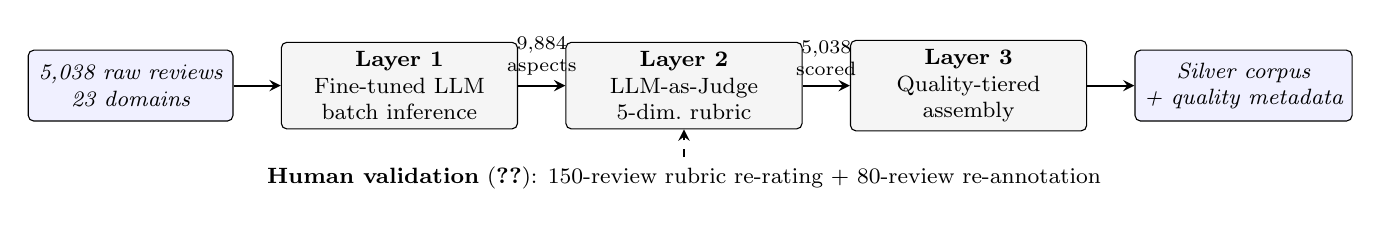
\begin{tikzpicture}[
  node distance=4mm and 6mm,
  stage/.style={draw, rounded corners=2pt, align=center, minimum height=11mm, minimum width=30mm, font=\footnotesize, fill=gray!8},
  data/.style={draw, rounded corners=2pt, align=center, minimum height=9mm, minimum width=26mm, font=\footnotesize\itshape, fill=blue!6},
  arrow/.style={-{stealth}, thick}
]
\node[data] (raw) {5{,}038 raw reviews\\23 domains};
\node[stage, right=of raw] (l1) {\textbf{Layer 1}\\Fine-tuned LLM\\batch inference};
\node[stage, right=of l1] (l2) {\textbf{Layer 2}\\LLM-as-Judge\\5-dim.\ rubric};
\node[stage, right=of l2] (l3) {\textbf{Layer 3}\\Quality-tiered\\assembly};
\node[data, right=of l3] (out) {Silver corpus\\+ quality metadata};
\draw[arrow] (raw) -- (l1);
\draw[arrow] (l1) -- (l2) node[midway, above, font=\scriptsize, align=center] {9{,}884\\aspects};
\draw[arrow] (l2) -- (l3) node[midway, above, font=\scriptsize, align=center] {5{,}038\\scored};
\draw[arrow] (l3) -- (out);
\node[below=3.5mm of l2, font=\footnotesize, align=center] (human) {\textbf{Human validation} (\cref{sec:res_human}): 150-review rubric re-rating + 80-review re-annotation};
\draw[arrow, dashed] (human.north) -- (l2.south);
\end{tikzpicture}%
}
\caption{Three-layer annotation pipeline. A locally fine-tuned LLM annotates the corpus, a panel of two LLM judges scores every review, and assembly assigns quality tiers. A native-speaker study (dashed) calibrates the judges.}
\label{fig:pipeline}
\end{figure}

\paragraph{Layer 1: annotation.} The fine-tuned Qwen model annotates all 5,038 reviews with greedy decoding and checkpointed batch inference, at roughly 4--5\,s per review on one RTX A6000 (about six GPU-hours in total). Qwen was chosen for its reliability: it is the only LLM with a 100\% parse rate and has the highest extraction recall among the LLMs (\cref{sec:res_compare}). The released annotations come from a Qwen checkpoint trained before the split and prompt-serialisation fixes of \cref{sec:res_loss}. That model never saw the Sharh corpus, so the annotations are not contaminated, but its benchmark scores under the earlier pipeline were lower (exact ATE F1 0.660 vs.\ 0.708). All quality figures in \cref{sec:res_domain,sec:res_human} are measured on the released annotations themselves.

\paragraph{Layer 2: judging.} Two LLM judges, GPT-4o-mini and GPT-4.1 (OpenAI API, accessed 30--31 October 2026; temperature 0.1, one call per review and judge), score every review on five 1--5 rubric dimensions: completeness, accuracy (extracted terms occur in the text), sentiment correctness, relevance (category--domain fit) and overall quality. The panel score is the mean of the two, since averaging several judges reduces the bias of any single one~\cite{verga2024juries}. All 10,076 responses parsed, at a measured cost of US\$10. A first round with GPT-4o-mini alone had scored a stratified sample of 307 reviews; \cref{sec:res_human} compares the two. The rubric prompt is released with the code.

\paragraph{Layer 3: tiering.} Every review is tiered by its panel overall score into \emph{Include} ($\ge$3.5), \emph{Flag} (2.5--3.5) and \emph{Exclude} ($<$2.5). The release includes per-dimension scores and provenance in JSON, and a JSONL export for the Hugging Face \texttt{datasets} library.

\section{Results}
\label{sec:results}

\subsection{Fine-Tuning versus Zero-Shot Prompting (RQ1)}
\label{sec:res_zs}

\begin{table}[t]
\centering
\caption{ABSA results on the 609 held-out reviews (737 gold terms). FT: fine-tuned; ZS: zero-shot. The best single fine-tuned score in each column is in bold; Vote: majority vote of the five fine-tuned systems (\cref{sec:res_compare}). Partial F1 uses one-to-one matching; Ratio: unique predicted aspects per gold term. 95\% bootstrap confidence intervals have half-widths of 0.023--0.037.}
\label{tab:main}
\setlength{\tabcolsep}{2.4pt}
\footnotesize
\begin{tabular}{@{}llccccccccc@{}}
\toprule
& & \multicolumn{3}{c}{\textbf{ATE exact}} & \textbf{ATE partial} & \textbf{Pair} & \multicolumn{2}{c}{\textbf{Sentiment}} & \textbf{Parse} & \\
\cmidrule(lr){3-5}\cmidrule(lr){8-9}
\textbf{System} & & P & R & F1 & F1 & F1 & Acc. & Macro-F1 & (\%) & \textbf{Ratio} \\
\midrule
Qwen 2.5-7B    & FT & 0.714 & 0.701 & \textbf{0.708} & \textbf{0.804} & 0.645 & 0.911 & 0.862 & \textbf{100.0} & 0.98 \\
Llama 3.1-8B   & FT & 0.719 & 0.689 & 0.704 & 0.802 & \textbf{0.651} & \textbf{0.925} & \textbf{0.887} & 97.4 & 0.96 \\
DeepSeek-R1-7B & FT & 0.714 & 0.645 & 0.678 & 0.789 & 0.603 & 0.891 & 0.831 & 96.9 & 0.90 \\
BERTbek        & FT & 0.680 & \textbf{0.704} & 0.692 & 0.799 & 0.608 & 0.879 & 0.813 & -- & 1.04 \\
TahrirchiBERT  & FT & \textbf{0.729} & 0.674 & 0.700 & 0.786 & 0.623 & 0.889 & 0.814 & -- & 0.93 \\
\midrule
Vote (5 systems) & FT & 0.800 & 0.707 & 0.751 & 0.821 & 0.690 & 0.919 & 0.870 & -- & 0.88 \\
\midrule
Qwen 2.5-7B    & ZS & 0.250 & 0.452 & 0.322 & 0.557 & 0.210 & 0.652 & 0.472 & 99.8 & 1.80 \\
Llama 3.1-8B   & ZS & 0.227 & 0.380 & 0.284 & 0.472 & 0.200 & 0.704 & 0.628 & 95.4 & 1.67 \\
DeepSeek-R1-7B & ZS & 0.208 & 0.227 & 0.217 & 0.279 & 0.154 & 0.713 & 0.568 & 46.3 & 1.10 \\
\bottomrule
\end{tabular}
\end{table}

\Cref{tab:main} compares each base model before and after adaptation, with the same prompt and decoding. Fine-tuning more than doubles exact ATE F1 (2.2--3.1$\times$) and more than triples pair F1 (3.1--3.9$\times$) for every model, all with $p<0.001$ after Holm correction; Qwen rises from 0.322 to 0.708 and from 0.210 to 0.645. The scores thus come from adaptation, not from latent Uzbek ABSA ability. Above all, fine-tuning teaches the models how much to extract: zero-shot Qwen already returns valid JSON for 99.8\% of reviews but predicts 1.80 aspects per gold term, against 0.90--0.98 after fine-tuning. For DeepSeek, zero-shot reasoning preambles break JSON parsing on more than half of the reviews (46.3\% parse rate), and fine-tuning raises the parse rate to 96.9\%.

\subsection{Comparison of Systems}
\label{sec:res_compare}

Qwen and Llama form the top tier. Qwen achieves the highest exact and partial ATE F1 (0.708 and 0.804) and is the only LLM with a 100\% parse rate; Llama achieves the highest pair F1 (0.651), sentiment accuracy (0.925) and macro-F1 (0.887). The two are statistically tied (exact ATE $p{=}0.79$, pair F1 $p{=}0.68$, sentiment accuracy $p{=}0.27$), and a second Qwen seed moves its exact ATE and pair F1 by $+0.002$ and $+0.011$, as much as the gaps between them, so either is a sound choice. DeepSeek trails both; its pair-F1 deficit to Llama ($-0.048$) is the only difference between fine-tuned systems that survives Holm correction (raw $p{=}0.0016$, adjusted $p{=}0.045$). Its deficit is under-extraction, not formatting: on the 589 reviews all three LLMs parse, it matches their precision (0.714 vs.\ 0.711--0.718) but has the lowest recall (0.672 vs.\ 0.698--0.716). Combining the systems pays off: a majority vote that keeps a term when at least three of the five fine-tuned systems predict it reaches 0.751 exact ATE F1 and 0.690 pair F1, above every single system on both metrics (10 of 10 comparisons significant after Holm correction, $p \le 0.034$), mainly through higher precision (0.800).

The comparison with the encoders separates the two subtasks. On extraction, a 110M-parameter monolingual encoder is competitive with the 7--8B LLMs: TahrirchiBERT reaches 0.700 exact F1 with the highest precision of all systems (0.729), BERTbek has the highest recall (0.704), and both are within 0.016 of Qwen ($p \ge 0.29$). On joint prediction and sentiment, Qwen and Llama score higher than both encoders on all three metrics (12 of 12 comparisons), by up to 4.3 pair-F1 and 7.4 macro-F1 points. Three of the six tested margins are significant at the 5\% level (Llama vs.\ TahrirchiBERT on sentiment accuracy, $p{=}0.014$; Qwen vs.\ BERTbek on pair F1 and sentiment accuracy, $p{=}0.020$ and $0.021$), although none survives correction over all 28 tests.

\subsection{Robustness of the Evaluation}
\label{sec:res_robust}

\begin{table}[t]
\centering
\caption{Sensitivity of F1 to the matching criterion (\cref{sec:eval}); best fine-tuned score per column in bold. Exact (set): canonical score of \cref{tab:main}; 1:1: maximum one-to-one matching; +Orth.: also normalising apostrophes, punctuation and spacing; +Stem: also stripping inflectional suffixes; ROUGE-L: soft character-level credit; Pair (stem): aspect--polarity F1 with stem-level matching.}
\label{tab:robust}
\setlength{\tabcolsep}{4.5pt}
\footnotesize
\begin{tabular}{@{}llcccccc@{}}
\toprule
& & \multicolumn{5}{c}{\textbf{ATE F1}} & \\
\cmidrule(lr){3-7}
\textbf{System} & & Exact (set) & Exact 1:1 & +Orth. & +Stem & ROUGE-L & \textbf{Pair (stem)} \\
\midrule
Qwen 2.5-7B    & FT & \textbf{0.708} & \textbf{0.708} & \textbf{0.715} & \textbf{0.716} & \textbf{0.806} & 0.652 \\
Llama 3.1-8B   & FT & 0.704 & 0.704 & 0.712 & 0.713 & 0.791 & \textbf{0.659} \\
DeepSeek-R1-7B & FT & 0.678 & 0.677 & 0.684 & 0.685 & 0.784 & 0.611 \\
BERTbek        & FT & 0.692 & 0.689 & 0.693 & 0.695 & 0.790 & 0.610 \\
TahrirchiBERT  & FT & 0.700 & 0.698 & 0.702 & 0.704 & 0.786 & 0.625 \\
\bottomrule
\end{tabular}
\end{table}

\paragraph{Matching criteria.} The leading systems keep their positions under every matching criterion (\cref{tab:robust}): Qwen has the highest ATE F1 under all five and Llama the highest pair F1 under both. No gold term repeats within a review, so set-based scoring discards none of the 737 gold terms, and one-to-one matching changes fine-tuned scores by at most 0.003. Orthographic normalisation adds 0.004--0.008, because some gold spans include trailing punctuation. Stemming adds at most 0.002 more for fine-tuned systems, which reproduce the inflected surface form of the gold term, but 0.026 for zero-shot Qwen, which tends to output uninflected forms (\textit{ofitsiant} for accusative \textit{ofitsiantni} `the waiter'). The gap of 0.09--0.11 between exact and partial F1 is therefore almost entirely span-boundary disagreement, such as included modifiers (\textit{biftek} vs.\ \textit{maxsus biftek} `special steak') or coordinated phrases (\textit{salat} vs.\ \textit{salat va uchta taom}), not inflection. Under stem-level matching, the paired tests of \cref{sec:res_compare} lead to the same conclusions (e.g., Qwen vs.\ Llama pair F1 $p{=}0.63$; Llama vs.\ DeepSeek $p<0.001$).

\paragraph{Re-checked gold.} Many apparent system errors are gold errors. Two native speakers (the author and a colleague) independently re-checked the 203 held-out reviews where the gold conflicts with the five fine-tuned systems, plus 60 random control reviews, blind to which candidate terms were gold ($\kappa$ 0.94 for aspects, 0.91 for polarity; 37 disagreements resolved by discussion). Of the 152 gold terms that at most one system predicts, 68\% were wrong and 52\% are not aspects at all (e.g., \textit{rahmat} `thank you'); 51\% of the 130 terms that most systems predict but the gold lacks are genuine aspects. The re-check changes 281 annotations in 169 reviews but only 4 of the 60 control reviews. On the re-checked gold every system gains 0.04--0.06 exact ATE F1 and 0.05--0.06 pair F1 (Qwen 0.770 and 0.702), and the tests reach the same conclusions (Qwen vs.\ Llama $p{=}0.21$ and $0.95$). As the reviews were chosen by disagreement, these scores complement \cref{tab:main}.


\subsection{Validation Loss and Data Splitting (RQ2)}
\label{sec:res_loss}

\begin{figure}[t]
\centering
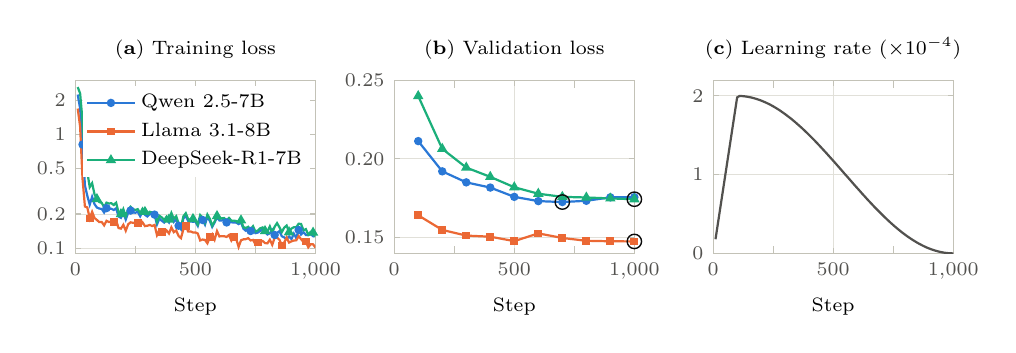
\begin{tikzpicture}
\begin{groupplot}[group style={group size=3 by 1, horizontal sep=10mm},
  paperaxis, scale only axis, width=3.05cm, height=2.2cm,
  xmin=0, xmax=1000, xtick={0,500,1000}, minor xtick={250,750}, xlabel={Step},
  every axis plot/.append style={line width=0.8pt}]
\nextgroupplot[title={(\textbf{a}) Training loss}, ymode=log, ymin=0.09, ymax=3,
  ytick={0.1,0.2,0.5,1,2}, log ticks with fixed point,
  legend cell align=left,
  legend style={font=\scriptsize, draw=none, fill=white, inner sep=1pt, at={(0.98,0.97)}, anchor=north east}]
\addplot[cQwen, mark=*, mark size=1.1pt, mark repeat=10, mark phase=3] coordinates {
  (10,2.2417) (20,1.6954) (30,0.8150) (40,0.3562) (50,0.2888) (60,0.2413) (70,0.2829) (80,0.2439) (90,0.2277) (100,0.2231)
  (110,0.2212) (120,0.2059) (130,0.2251) (140,0.2215) (150,0.2220) (160,0.2167) (170,0.2243) (180,0.1902) (190,0.1849) (200,0.2047)
  (210,0.1786) (220,0.2048) (230,0.2142) (240,0.2071) (250,0.2049) (260,0.2087) (270,0.1909) (280,0.2099) (290,0.1965) (300,0.1901)
  (310,0.2003) (320,0.1981) (330,0.1973) (340,0.1616) (350,0.1817) (360,0.1744) (370,0.1681) (380,0.1785) (390,0.1684) (400,0.1919)
  (410,0.1704) (420,0.1800) (430,0.1576) (440,0.1469) (450,0.1822) (460,0.1920) (470,0.1731) (480,0.1715) (490,0.1710) (500,0.1713)
  (510,0.1569) (520,0.1854) (530,0.1769) (540,0.1610) (550,0.1902) (560,0.1739) (570,0.1539) (580,0.1685) (590,0.1869) (600,0.1754)
  (610,0.1750) (620,0.1790) (630,0.1684) (640,0.1765) (650,0.1690) (660,0.1680) (670,0.1677) (680,0.1630) (690,0.1685) (700,0.1484)
  (710,0.1423) (720,0.1486) (730,0.1416) (740,0.1479) (750,0.1355) (760,0.1372) (770,0.1423) (780,0.1462) (790,0.1380) (800,0.1320)
  (810,0.1353) (820,0.1448) (830,0.1306) (840,0.1361) (850,0.1412) (860,0.1272) (870,0.1242) (880,0.1208) (890,0.1266) (900,0.1202)
  (910,0.1341) (920,0.1228) (930,0.1446) (940,0.1319) (950,0.1385) (960,0.1308) (970,0.1306) (980,0.1329) (990,0.1277) (1000,0.1376)};
\addlegendentry{Qwen 2.5-7B}
\addplot[cLlama, mark=square*, mark size=1.0pt, mark repeat=10, mark phase=6] coordinates {
  (10,1.6890) (20,1.1741) (30,0.4081) (40,0.2326) (50,0.2282) (60,0.1827) (70,0.2089) (80,0.1841) (90,0.1770) (100,0.1695)
  (110,0.1699) (120,0.1588) (130,0.1741) (140,0.1699) (150,0.1716) (160,0.1695) (170,0.1757) (180,0.1504) (190,0.1486) (200,0.1605)
  (210,0.1424) (220,0.1620) (230,0.1687) (240,0.1673) (250,0.1661) (260,0.1661) (270,0.1583) (280,0.1686) (290,0.1564) (300,0.1576)
  (310,0.1601) (320,0.1566) (330,0.1601) (340,0.1304) (350,0.1443) (360,0.1397) (370,0.1353) (380,0.1432) (390,0.1346) (400,0.1523)
  (410,0.1383) (420,0.1432) (430,0.1281) (440,0.1226) (450,0.1468) (460,0.1561) (470,0.1401) (480,0.1404) (490,0.1375) (500,0.1377)
  (510,0.1346) (520,0.1169) (530,0.1192) (540,0.1181) (550,0.1104) (560,0.1248) (570,0.1325) (580,0.1189) (590,0.1414) (600,0.1268)
  (610,0.1277) (620,0.1274) (630,0.1256) (640,0.1306) (650,0.1166) (660,0.1256) (670,0.1209) (680,0.1026) (690,0.1174) (700,0.1196)
  (710,0.1201) (720,0.1226) (730,0.1170) (740,0.1182) (750,0.1084) (760,0.1121) (770,0.1153) (780,0.1157) (790,0.1109) (800,0.1103)
  (810,0.1188) (820,0.1071) (830,0.1235) (840,0.1238) (850,0.1187) (860,0.1058) (870,0.1123) (880,0.1243) (890,0.1121) (900,0.1150)
  (910,0.1169) (920,0.1172) (930,0.1276) (940,0.1200) (950,0.1133) (960,0.1146) (970,0.1018) (980,0.1085) (990,0.1081) (1000,0.1013)};
\addlegendentry{Llama 3.1-8B}
\addplot[cDeepSeek, mark=triangle*, mark size=1.4pt, mark repeat=10, mark phase=9] coordinates {
  (10,2.6082) (20,2.2966) (30,1.3252) (40,0.6640) (50,0.4676) (60,0.3444) (70,0.3728) (80,0.2974) (90,0.2702) (100,0.2540)
  (110,0.2504) (120,0.2292) (130,0.2515) (140,0.2471) (150,0.2484) (160,0.2398) (170,0.2512) (180,0.2071) (190,0.1993) (200,0.2208)
  (210,0.1910) (220,0.2187) (230,0.2315) (240,0.2210) (250,0.2166) (260,0.2204) (270,0.2039) (280,0.2229) (290,0.2084) (300,0.2001)
  (310,0.2090) (320,0.2060) (330,0.2074) (340,0.1700) (350,0.1927) (360,0.1865) (370,0.1766) (380,0.1894) (390,0.1787) (400,0.2042)
  (410,0.1812) (420,0.1909) (430,0.1651) (440,0.1529) (450,0.1904) (460,0.2029) (470,0.1802) (480,0.1780) (490,0.1807) (500,0.1749)
  (510,0.1614) (520,0.1955) (530,0.1851) (540,0.1671) (550,0.1978) (560,0.1819) (570,0.1578) (580,0.1714) (590,0.1917) (600,0.1811)
  (610,0.1833) (620,0.1840) (630,0.1746) (640,0.1845) (650,0.1745) (660,0.1747) (670,0.1733) (680,0.1700) (690,0.1756) (700,0.1531)
  (710,0.1504) (720,0.1542) (730,0.1468) (740,0.1561) (750,0.1400) (760,0.1431) (770,0.1495) (780,0.1522) (790,0.1415) (800,0.1401)
  (810,0.1555) (820,0.1370) (830,0.1545) (840,0.1661) (850,0.1527) (860,0.1386) (870,0.1518) (880,0.1581) (890,0.1381) (900,0.1489)
  (910,0.1527) (920,0.1530) (930,0.1641) (940,0.1632) (950,0.1439) (960,0.1472) (970,0.1315) (980,0.1393) (990,0.1370) (1000,0.1255)};
\addlegendentry{DeepSeek-R1-7B}
\nextgroupplot[title={(\textbf{b}) Validation loss}, ymin=0.14, ymax=0.25, ytick={0.15,0.20,0.25},
  yticklabel style={/pgf/number format/fixed, /pgf/number format/precision=2, /pgf/number format/fixed zerofill}]
\addplot[cQwen, mark=*, mark size=1.1pt] coordinates {
  (100,0.2113) (200,0.1921) (300,0.1851) (400,0.1818) (500,0.1759) (600,0.1732) (700,0.1726) (800,0.1734) (900,0.1756) (1000,0.1757)};
\addplot[cLlama, mark=square*, mark size=1.0pt] coordinates {
  (100,0.1642) (200,0.1549) (300,0.1513) (400,0.1506) (500,0.1478) (600,0.1527) (700,0.1498) (800,0.1480) (900,0.1477) (1000,0.1476)};
\addplot[cDeepSeek, mark=triangle*, mark size=1.4pt] coordinates {
  (100,0.2399) (200,0.2064) (300,0.1945) (400,0.1886) (500,0.1820) (600,0.1779) (700,0.1759) (800,0.1755) (900,0.1749) (1000,0.1744)};
% checkpoints kept for evaluation (lowest validation loss)
\addplot[only marks, mark=o, mark size=2.6pt, cInk, line width=0.5pt] coordinates {(700,0.1726) (1000,0.1476) (1000,0.1744)};
\nextgroupplot[title={(\textbf{c}) Learning rate ($\times 10^{-4}$)}, ymin=0, ymax=2.2, ytick={0,1,2}]
\addplot[cInk2, no markers] coordinates {
  (10,0.180) (20,0.380) (30,0.580) (40,0.780) (50,0.980) (60,1.180) (70,1.380) (80,1.580) (90,1.780) (100,1.980)
  (110,2.000) (120,1.998) (130,1.995) (140,1.991) (150,1.985) (160,1.979) (170,1.971) (180,1.962) (190,1.952) (200,1.941)
  (210,1.928) (220,1.915) (230,1.900) (240,1.885) (250,1.868) (260,1.850) (270,1.831) (280,1.811) (290,1.790) (300,1.768)
  (310,1.745) (320,1.722) (330,1.697) (340,1.672) (350,1.645) (360,1.618) (370,1.591) (380,1.562) (390,1.533) (400,1.503)
  (410,1.473) (420,1.442) (430,1.410) (440,1.378) (450,1.345) (460,1.312) (470,1.279) (480,1.245) (490,1.211) (500,1.177)
  (510,1.143) (520,1.108) (530,1.073) (540,1.038) (550,1.003) (560,0.969) (570,0.934) (580,0.899) (590,0.864) (600,0.830)
  (610,0.796) (620,0.761) (630,0.728) (640,0.694) (650,0.661) (660,0.629) (670,0.596) (680,0.565) (690,0.534) (700,0.503)
  (710,0.473) (720,0.444) (730,0.415) (740,0.387) (750,0.360) (760,0.333) (770,0.308) (780,0.283) (790,0.259) (800,0.236)
  (810,0.214) (820,0.193) (830,0.173) (840,0.154) (850,0.136) (860,0.119) (870,0.103) (880,0.088) (890,0.074) (900,0.062)
  (910,0.050) (920,0.040) (930,0.031) (940,0.023) (950,0.016) (960,0.010) (970,0.006) (980,0.003) (990,0.001) (1000,0.000)};
\end{groupplot}
\end{tikzpicture}
\caption{Fine-tuning dynamics: (\textbf{a})~training loss (log scale), (\textbf{b})~validation loss, with rings at the checkpoints kept for evaluation, and (\textbf{c})~the shared learning-rate schedule. Qwen and DeepSeek end with almost equal validation loss but different task scores (\cref{tab:main}), whereas Llama's clearly lower loss brings no significant gain over Qwen.}
\label{fig:loss}
\end{figure}

\paragraph{Validation loss misranks models.} Llama reaches the lowest validation loss (0.148), while Qwen and DeepSeek finish almost level (0.173 vs.\ 0.174; \cref{fig:loss}b), yet Qwen leads DeepSeek by 0.030 exact ATE F1 and 0.041 pair F1 (raw $p{=}0.009$). Cross-entropy weights every token, including JSON punctuation, and does not reward correct span boundaries or polarities as such. For structured extraction, models and checkpoints should therefore be selected on held-out task metrics rather than on loss.

\paragraph{Leakage-free splitting raises scores.} Short formulaic reviews (\textit{mazali} `tasty', \textit{ajoyib} `excellent') recur verbatim, and the term and category records of one review are stored separately, so a naive record-level split leaks: in an earlier pipeline revision, 61 of the 609 held-out items (10.0\%) had an exact-text twin in training. The review-grouped split raised every system's scores, by 0.023--0.074 exact ATE F1 and 0.047--0.102 pair F1 (largest for DeepSeek, smallest for BERTbek; the LLM changes also include a prompt-serialisation fix). Leakage depressed rather than inflated the scores because a model that saw an eval-identical text with only one annotation layer as its target learned to reproduce that partial answer.

\subsection{Multi-Domain Annotation (RQ3)}
\label{sec:res_domain}

The fine-tuned model annotates all 5,038 reviews with a 100\% parse rate, producing 9,884 aspects (1.96 per review; 75.1\% positive, 16.5\% negative, 8.4\% neutral). \textit{Boshqalar} (other) is the most frequent category (45.5\%), ahead of \textit{ovqat} (17.9\%), \textit{xizmat} (15.9\%), \textit{muhit} (10.7\%) and \textit{narx} (9.0\%). The judge panel rates the annotations highly for accuracy (4.50 of 5) and sentiment (4.24), so the model rarely invents aspects or misreads polarity; its main weakness is completeness (3.36), that is, missed opinions. Of all 5,038 reviews, 3,608 (71.6\%) reach Include and only 458 (9.1\%) are excluded.

\begin{figure}[t]
\centering
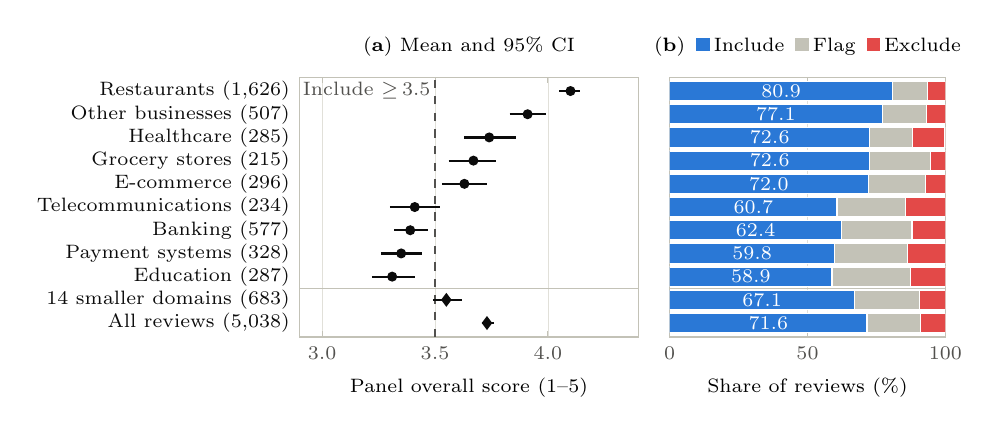
\begin{tikzpicture}
\begin{groupplot}[group style={group size=2 by 1, horizontal sep=4mm},
  paperaxis, scale only axis, height=3.3cm, ymin=0.4, ymax=11.6, ytick={1,...,11},
  ymajorgrids=false, ytick style={draw=none}]
\nextgroupplot[width=4.3cm, xmin=2.9, xmax=4.4, xtick={3,3.5,4},
  xticklabel style={/pgf/number format/fixed, /pgf/number format/precision=1, /pgf/number format/fixed zerofill},
  xlabel={Panel overall score (1--5)}, title={(\textbf{a}) Mean and 95\% CI},
  yticklabels={{All reviews (5,038)}, 14 smaller domains (683), Education (287),
    Payment systems (328), Banking (577), Telecommunications (234), E-commerce (296),
    Grocery stores (215), Healthcare (285), Other businesses (507), {Restaurants (1,626)}},
  yticklabel style={color=cInk}]
\draw[cInk2, dashed, line width=0.5pt] (axis cs:3.5,0.4) -- (axis cs:3.5,11.6);
\node[font=\scriptsize, text=cInk2, anchor=north east, inner sep=1.5pt] at (axis cs:3.5,11.6) {Include $\geq$\,3.5};
\draw[cAxis, line width=0.3pt] (axis cs:2.9,2.5) -- (axis cs:4.4,2.5);
% 95% bootstrap confidence intervals (experiments/v3/results/judge_paper_numbers.json, domains.groups)
\draw[cInk, line width=0.8pt] (axis cs:4.05,11) -- (axis cs:4.14,11);
\draw[cInk, line width=0.8pt] (axis cs:3.83,10) -- (axis cs:3.99,10);
\draw[cInk, line width=0.8pt] (axis cs:3.63,9) -- (axis cs:3.86,9);
\draw[cInk, line width=0.8pt] (axis cs:3.56,8) -- (axis cs:3.77,8);
\draw[cInk, line width=0.8pt] (axis cs:3.53,7) -- (axis cs:3.73,7);
\draw[cInk, line width=0.8pt] (axis cs:3.30,6) -- (axis cs:3.52,6);
\draw[cInk, line width=0.8pt] (axis cs:3.32,5) -- (axis cs:3.47,5);
\draw[cInk, line width=0.8pt] (axis cs:3.26,4) -- (axis cs:3.44,4);
\draw[cInk, line width=0.8pt] (axis cs:3.22,3) -- (axis cs:3.41,3);
\draw[cInk, line width=0.8pt] (axis cs:3.49,2) -- (axis cs:3.62,2);
\draw[cInk, line width=0.8pt] (axis cs:3.71,1) -- (axis cs:3.76,1);
\addplot[only marks, mark=*, mark size=1.6pt, cInk] coordinates {
  (4.10,11) (3.91,10) (3.74,9) (3.67,8) (3.63,7) (3.41,6) (3.39,5) (3.35,4) (3.31,3)};
\addplot[only marks, mark=diamond*, mark size=2.2pt, cInk] coordinates {(3.55,2) (3.73,1)};
\nextgroupplot[width=3.5cm, xmin=0, xmax=100, xtick={0,50,100}, xlabel={Share of reviews (\%)},
  title={(\textbf{b})\enspace\tierkey{cInclude}\,Include\enspace\tierkey{cFlag}\,Flag\enspace\tierkey{cExclude}\,Exclude},
  xbar stacked, bar width=7pt, yticklabels={}]
\addplot[fill=cInclude, draw=white, line width=0.4pt, point meta=x, nodes near coords,
  nodes near coords style={font=\scriptsize, text=white, anchor=center, inner sep=0pt,
    /pgf/number format/fixed, /pgf/number format/precision=1, /pgf/number format/fixed zerofill}]
  coordinates {(71.6,1) (67.1,2) (58.9,3) (59.8,4) (62.4,5) (60.7,6) (72.0,7) (72.6,8) (72.6,9) (77.1,10) (80.9,11)};
\addplot[fill=cFlag, draw=white, line width=0.4pt]
  coordinates {(19.3,1) (23.4,2) (28.6,3) (26.5,4) (25.5,5) (24.8,6) (20.9,7) (21.9,8) (15.4,9) (16.2,10) (12.5,11)};
\addplot[fill=cExclude, draw=white, line width=0.4pt]
  coordinates {(9.1,1) (9.5,2) (12.5,3) (13.7,4) (12.1,5) (14.5,6) (7.1,7) (5.6,8) (11.9,9) (6.7,10) (6.6,11)};
\draw[cAxis, line width=0.3pt] (axis cs:0,2.5) -- (axis cs:100,2.5);
\end{groupplot}
\end{tikzpicture}
\caption{Judge-panel overall scores by domain for all 5,038 reviews (reviews in parentheses; restaurants are the training domain; the 14 smallest domains, with 7--173 reviews each, are pooled): (\textbf{a})~mean with 95\% bootstrap confidence interval and the Include threshold of 3.5; (\textbf{b})~share of reviews per quality tier, labelled with the Include share.}
\label{fig:domains}
\end{figure}

The model transfers well beyond its training domain (\cref{fig:domains}): in all nine out-of-domain groups most reviews reach the Include tier (58.9--77.1\%), as they do in 20 of the 22 individual out-of-domain domains. Quality is highest in the training domain (mean 4.10, 95\% CI [4.05, 4.14]; 80.9\% Include), and the intervals of other businesses, healthcare, grocery stores and e-commerce also lie above the threshold; education (3.31) and payment systems (3.35) are the hardest of the large domains. Accuracy is at least 4.08 in every domain: the decline comes from missed aspects, not invented ones.

Script matters more than domain: the 152 reviews in Uzbek Cyrillic, which the training data lacks, reach Include less often (50.0\%) than any domain group. Transliterating them to Latin before annotation and mapping the terms back raises their Include rate from 54.6\% to 68.4\% with the corrected Qwen model (31 reviews enter Include, 10 leave it; McNemar $p{=}0.002$).

\subsection{Human Validation}
\label{sec:res_human}

Two native Uzbek speakers, the author and a second annotator, rated the annotations of 150 of the 307 reviews of the first judging round (all 23 domains, oversampling distant and low-scoring ones) on the judges' rubric, and re-annotated 80 of them from scratch. After a joint calibration pass, agreement is almost perfect on every dimension (quadratic-weighted $\kappa$ 0.911--0.970, \cref{tab:human}), so the mean human rating is the reference.

\begin{table}[t]
\centering
\caption{Human validation on 150 reviews: inter-annotator agreement (IAA; quadratic-weighted $\kappa$, interval Krippendorff's $\alpha$) and judge calibration against the mean human rating: Spearman $\rho$ of the first-round single judge and of the two-judge panel (all $p<10^{-6}$), and the panel's MAE on the 1--5 scale.}
\label{tab:human}
\setlength{\tabcolsep}{6pt}
\footnotesize
\begin{tabular}{@{}lccccc@{}}
\toprule
& \multicolumn{2}{c}{\textbf{IAA}} & \multicolumn{3}{c}{\textbf{Judge vs.\ humans}} \\
\cmidrule(lr){2-3}\cmidrule(lr){4-6}
\textbf{Dimension} & $\kappa_w$ & $\alpha$ & $\rho$ single & $\rho$ panel & MAE \\
\midrule
Sentiment    & 0.970 & 0.970 & 0.806 & \textbf{0.857} & 0.25 \\
Relevance    & 0.911 & 0.911 & 0.667 & \textbf{0.774} & 0.43 \\
Overall      & 0.923 & 0.922 & 0.657 & \textbf{0.781} & 0.48 \\
Completeness & 0.930 & 0.930 & 0.462 & \textbf{0.636} & 0.84 \\
Accuracy     & 0.936 & 0.936 & 0.433 & \textbf{0.560} & 0.48 \\
\bottomrule
\end{tabular}
\end{table}

\begin{figure}[t]
\centering
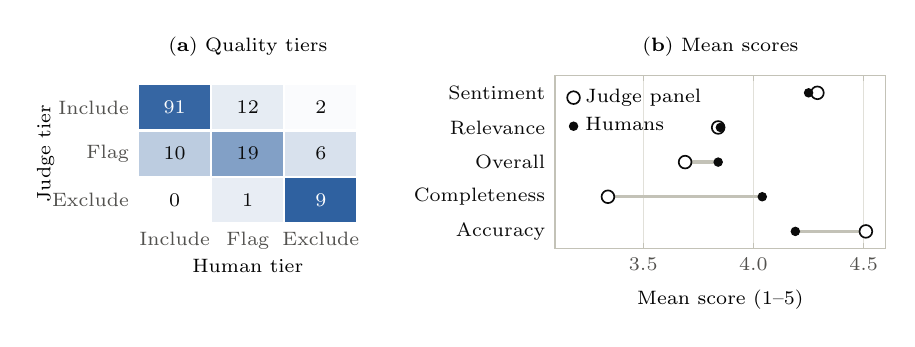
\begin{tikzpicture}
% (a) tier confusion matrix (experiments/v3/results/judge_paper_numbers.json,
% calibration.panel_in_corpus_run.tiers.confusion_rows_judge_cols_human); shading = row share
\matrix (cm) [matrix of nodes, column sep=0.8pt, row sep=0.8pt,
  nodes={minimum width=9mm, minimum height=5.6mm, inner sep=0pt, font=\scriptsize, text=cInk}] {
  |[fill=cSeq!87!white, text=white]| 91 & |[fill=cSeq!11!white]| 12 & |[fill=cSeq!2!white]| 2 \\
  |[fill=cSeq!29!white]| 10 & |[fill=cSeq!54!white]| 19 & |[fill=cSeq!17!white]| 6 \\
  |[fill=white]| 0 & |[fill=cSeq!10!white]| 1 & |[fill=cSeq!90!white, text=white]| 9 \\
};
\foreach \i/\t in {1/Include, 2/Flag, 3/Exclude} {
  \node[font=\scriptsize, text=cInk2, anchor=north] at (cm-3-\i.south) {\t};
  \node[font=\scriptsize, text=cInk2, anchor=east] at (cm-\i-1.west) {\t};
}
\node[font=\scriptsize, anchor=north] at ($(cm-3-2.south)+(0,-3.4mm)$) {Human tier};
\node[font=\scriptsize, rotate=90, anchor=south] at ($(cm-2-1.west)+(-9.5mm,0)$) {Judge tier};
\node[font=\scriptsize, anchor=south] at ($(cm.north)+(0,1.2mm)$) {(\textbf{a}) Quality tiers};
% (b) mean scores per rubric dimension
\begin{axis}[name=dumb, paperaxis, at={($(cm.north east)+(24mm,0)$)}, anchor=north west,
  scale only axis, width=4.2cm, height=2.2cm, xmin=3.1, xmax=4.6, xtick={3.5,4,4.5},
  xticklabel style={/pgf/number format/fixed, /pgf/number format/precision=1, /pgf/number format/fixed zerofill},
  xlabel={Mean score (1--5)}, ymin=0.5, ymax=5.5, ytick={1,...,5},
  yticklabels={Accuracy, Completeness, Overall, Relevance, Sentiment}, yticklabel style={color=cInk},
  ymajorgrids=false, ytick style={draw=none}, legend cell align=left,
  legend style={font=\scriptsize, draw=none, fill=none, at={(0.01,0.99)}, anchor=north west}]
\draw[cAxis, line width=1.2pt] (axis cs:4.19,1) -- (axis cs:4.51,1);
\draw[cAxis, line width=1.2pt] (axis cs:4.04,2) -- (axis cs:3.34,2);
\draw[cAxis, line width=1.2pt] (axis cs:3.84,3) -- (axis cs:3.69,3);
\draw[cAxis, line width=1.2pt] (axis cs:3.85,4) -- (axis cs:3.84,4);
\draw[cAxis, line width=1.2pt] (axis cs:4.25,5) -- (axis cs:4.29,5);
\addplot[only marks, mark=*, mark size=2.3pt, mark options={fill=white, draw=cInk, line width=0.6pt}]
  coordinates {(4.51,1) (3.34,2) (3.69,3) (3.84,4) (4.29,5)};
\addlegendentry{Judge panel}
\addplot[only marks, mark=*, mark size=1.5pt, cInk] coordinates {(4.19,1) (4.04,2) (3.84,3) (3.85,4) (4.25,5)};
\addlegendentry{Humans}
\end{axis}
\node[font=\scriptsize, anchor=south] at ($(dumb.north)+(0,1.2mm)$) {(\textbf{b}) Mean scores};
\end{tikzpicture}
\caption{Judge calibration on the 150 human-rated reviews: (\textbf{a})~tiers from the panel's overall score (rows) and from the mean human rating under the same thresholds (columns), shaded by row share; (\textbf{b})~mean scores per rubric dimension.}
\label{fig:judge}
\end{figure}

\paragraph{Judge calibration.} The judge panel is a dependable quality filter. Passing the mean human overall rating through the same thresholds, panel and human tiers coincide for 79.3\% of the reviews (Cohen's $\kappa{=}0.56$; linear-weighted 0.63; \cref{fig:judge}a), against 73.3\% ($\kappa{=}0.47$) for GPT-4o-mini alone in the first round. Of the reviews the panel includes, 86.7\% are included by the humans as well, and severe errors are rare: only 2 of the 150 reviews are Include on one side and Exclude on the other. The panel also ranks reviews more like the humans ($\rho{=}0.78$ vs.\ 0.66 on the overall score, paired bootstrap $p{<}0.001$; for $\kappa$, $p{=}0.08$), most on completeness (0.64 vs.\ 0.46; \cref{tab:human}), and a repeat run put 95\% of the reviews in the same tier. Means agree on the tier-defining overall score (3.69 vs.\ 3.84; \cref{fig:judge}b); the panel is stricter than the humans on completeness (3.34 vs.\ 4.04) and more lenient on accuracy (4.51 vs.\ 4.19), so tiers use the overall score alone.

\paragraph{Re-annotation.} On the 80 re-annotated reviews, the model agrees with the annotators about as well as they first agreed with each other: its partial F1 against each annotator's reconciled annotations is 0.425--0.433 (exact 0.209--0.224), against a first-pass inter-annotator agreement of 0.415 (exact 0.277), and its polarity matches theirs on every exactly matched term. The annotators' low first-pass span agreement reflected different conventions (lemma vs.\ surface form, referent vs.\ mention), not different opinions; once these were reconciled, they reached 0.927 exact F1 with 100\% polarity agreement. We release it as a reconciled double-annotated subset. The model's exact pair F1 on it is 0.244 for general out-of-domain reviews and 0.170 for the most distant domains, so span conventions, not sentiment, are the main open problem.

\section{Discussion and Limitations}
\label{sec:discussion}

\paragraph{Which model to use?} For aspect extraction alone, a monolingual encoder trained in ten minutes on a laptop is competitive with 7--8B LLMs. When polarity, categories or new domains matter, a QLoRA-tuned LLM is the stronger choice: Qwen and Llama lead on joint prediction and sentiment by up to 4.3 pair-F1 points, emit term- and category-level output in a single pass, and follow instructions on unseen domains, which the annotation pipeline relies on. Models and checkpoints should be chosen on task metrics, not on validation loss. The comparison contrasts two practical recipes rather than isolating a cause, since parameter count, quantisation, tokenizer and pre-training data all differ.

\paragraph{Where the remaining errors are.} Completeness is the main lever for improvement: the five UzABSA categories do not cover many out-of-domain aspects, which the model maps to \textit{boshqalar} (45.5\% of predicted categories). Multi-domain fine-tuning with the released sub-aspect taxonomy is a natural remedy, with the human-validated subset as its test set. Span segmentation, not polarity, is the dominant source of disagreement both between annotators and between model and humans, which argues for training and evaluation that are explicit about span conventions.

\paragraph{Limitations.} (i)~Checkpoints were selected on the held-out set (\cref{sec:eval}), so scores may be mildly optimistic; a three-way split is planned. (ii)~Seed variance is measured only for Qwen ($\pm$0.01 F1). (iii)~One QLoRA configuration was used, and few-shot prompting and schema-constrained decoding were not evaluated. (iv)~The \textit{conflict} class is excluded, and term--category triplets are not evaluated because UzABSA does not link the two layers. (v)~The judge panel and rubric were chosen on the same 150 ratings that evaluate them (a longer checklist prompt agreed less), so their agreement may be slightly optimistic; the stemmer is rule-based rather than a full morphological analyser~\cite{Salaev2024}; and the silver labels predate the corrected annotator (\cref{sec:pipeline}); a regenerated release is planned.

\section{Conclusion}
\label{sec:conclusion}

QLoRA fine-tuning turns open-weight 7--8B LLMs into strong Uzbek ABSA systems on a single GPU, more than doubling exact aspect-extraction F1 and tripling aspect--polarity pair F1 over zero-shot prompting. Qwen~2.5-7B and Llama~3.1-8B form a statistically tied top tier that scores higher than fine-tuned Uzbek BERT encoders on every joint and sentiment metric, while the encoders remain a cheap and competitive choice for extraction alone. These results hold under one-to-one and morphology-aware matching, and validation loss proves an unreliable guide for model selection. Trained only on restaurant reviews, the model annotates 23 business domains with a perfect parse rate, and a two-judge LLM panel calibrated against native speakers turns its output into a fully quality-tiered resource in which 72\% of the reviews reach the highest tier. Future work includes a three-way split with multi-seed runs, triplet annotation, domain-adaptive fine-tuning, and syntax-aware extraction that uses Uzbek UD resources~\cite{MATLATIPOV2026112857,11632281}, since span segmentation is where models and humans disagree most.

\begin{credits}
\subsubsection{\ackname} The author thanks Sardor Berdiyev, CEO and co-founder of Commeta, for permission to use publicly available reviews from the sharh.commeta.uz platform exclusively for academic research; Jaloliddin Rajabov, the second annotator in the human validation and the test-set re-check; and the National University of Uzbekistan for computational resources.

\subsubsection{\discintname} The author has no competing interests to declare that are relevant to the content of this article.
\end{credits}
%
% ---- Bibliography ----
%
% BibTeX users should specify bibliography style 'splncs04'.
% References will then be sorted and formatted in the correct style.
%
\bibliographystyle{splncs04}
\bibliography{mybibliography}
%
\end{document}
